\documentclass[12pt, a4paper, oneside]{article}
\usepackage{amsmath, amsthm, amssymb, bm, graphicx, hyperref, mathrsfs}
\usepackage{geometry}
\usepackage{amsmath}
\newtheorem{theorem}{Theorem}
\newtheorem{lemma}{Lemma}
\usepackage{hyperref}
\usepackage{mathrsfs}
\usepackage[ruled, lined, linesnumbered, commentsnumbered, longend]{algorithm2e}
\usepackage{booktabs}
\usepackage{breqn}
\usepackage{natbib}
\usepackage{amsmath}
\numberwithin{equation}{section}
\usepackage[ruled,linesnumbered]{algorithm2e}
\usepackage[UTF8]{ctex}
\usepackage{subfigure}

\title{\textbf{Hierarchical heterogeneous analysis of high-dimensional data
		based on interactions (Test Part)}}
\author{Yan Ren \\ 2021103739}
\date{\today}
\linespread{1.5}
\newcounter{problemname}
\newenvironment{problem}{\stepcounter{problemname}\par\noindent\textsc{Problem \arabic{problemname}. }}{\\\par}
\newenvironment{solution}{\par\noindent\textsc{Solution. }}{\\\par}
\newenvironment{note}{\par\noindent\textsc{Note of Problem \arabic{problemname}. }}{\\\par}
\newcommand{\nysm}{Nystr$\ddot{\rm o}$m Method}
\geometry{a4paper, scale = 0.8}

\begin{document}
	
\maketitle
\newpage
\tableofcontents
\newpage

\section{Simple Set1-Linear}
\label{subsec:test-set1}

\subsection{Estimation}

尝试最简单的设定验证代码的准确性,模型简化为多分类的回归问题,在类别内部有

\begin{equation}
	Y_i = X_i^T \beta_k, \text{ if } i \in \text{ Class }k
\end{equation}

目标函数现简化为 minimize 负对数似然函数

\begin{equation}
	l = -log P_Y (y)  = -\sum_{i = 1}^{n} log\sum_{k=1}^K \pi_k f_k(y_i|X_i,\beta_k)
\end{equation}

引入 hidden varaible $C_i$ 用以指示第 $i$ 个样本所属类别,其后验分布分布列为

\begin{equation}
	q_{C_i}(c_i) = \frac{\displaystyle\prod_{k=1}^{K}{\left(\pi_k f_k(y_i)\right)^{I(C_i=k)}}}{\displaystyle\sum_{k=1}^{K}\pi_{k^\prime} f_{k^\prime}(y_i)}
\end{equation}

进而(根据[Gaussian mixture models and the EM algorithm])

\begin{equation}
	\begin{aligned}
	log_Y (y)  &= log \sum_{k = 1}^{K}p_{Y,C}(y,c) \\
	&= log E_{q_C}\left(\frac{p_{Y,C}(y,c)}{q_C(c)}\right) \\
	&\geq E_{q_C}\left(\frac{p_{Y,C}(y,c)}{q_C(c)}\right) \\
	&= E_{q_C} \left(log p_{Y,C}(y,c)\right) - E_{q_C}\left(log q_C(c)\right)
	\end{aligned}
\end{equation}

其中 $E_{q_C}\left(log q_C(c)\right)$ 与 $\beta_k$ 取值无关,对参数进行估计时仅考虑第一项,此时问题转化为最大化 $E_{q_C} log p_{Y,C}(y,c)$

\begin{equation}
	\begin{aligned}
		E_{q_C}log p_{Y,C}(y,k) &= E_{q_C} log \left(p_C(c) p_{Y|C}(y)\right)\\
		&= E_{q_C} log \left(\prod^{n}_{i=1} p_{C_i}(c_i) p_{Y_i|C_i}(y_i) \right) \\
		&= E_{q_C} log \left(\prod^{n}_{i=1}\prod^{K}_{k=1} \pi_{c_i} f_{Y_i|C_i}(y_i) \right)^{I(C_i=k)} \\
		&= E_{q_C} \sum^{n}_{i=1}\sum^{K}_{k=1} I(C_i=k)\left( log\pi_{c_i} + log f_{Y_i|C_i}(y_i) \right) \\
		&= \sum^{n}_{i=1}\sum^{K}_{k=1} E_{q_C} I(C_i=k)\left( log\pi_{c_i} + log f_{Y_i|C_i}(y_i) \right) \\
		&= \sum^{n}_{i=1}\sum^{K}_{k=1} q_{C_i}(k)\left( log\pi_{c_i} + log f_{Y_i|C_i}(y_i) \right) \\
		&= \sum^{n}_{i=1}\sum^{K}_{k=1} q_{C_i}(k)\left( log\pi_{c_i} + log \rho_k - \frac{1}{2} log 2\pi - \frac{\rho_k^2}{2}(y_i - \mu_{ik})^2 \right) 
	\end{aligned}
\label{eq:l}
\end{equation}

其中 $C$ 为与参数无关的项,对于类别 $k$,优化目标为

\begin{equation}
	\text{max}\qquad \displaystyle\sum_{i=1}^{n}q_{C_i}(k)\left(C-\frac{\rho_k^2}{2}(y_i - X_i^T \beta_k)^2 \right)
\end{equation}
$\iff$
\begin{equation}
	\begin{aligned}
		\text{min}\qquad l_k &=  \displaystyle\sum_{i=1}^{n}q_{C_i}(k)\left(y_i - X_i^T \beta_k\right)^2 \\
		&= (y - X\beta_k)^T W_k (y - X\beta_k)
	\end{aligned}
\end{equation}
其中 $W_k = diag(q_{C_1}(k),...,q_{C_n}(k))$, $y = (y_1,...,y_n)^T\in \mathbb{R}^{n\times 1}$, $X = (X_1, ..., X_n)^T\in \mathbb{R}^{n\times p}$, $\beta_k \in \mathbb{R}^{p\times 1}$

转化为加权最小二乘问题(文献 \cite{wls} page 3),解为
\begin{equation}
	\hat \beta_k = (X^T W_k X)^{-1}X^T W_k y
\end{equation}

$\rho_k$ 的选取会对分类效果产生影响。可以认为各类别共用一个 $\rho$(即认为各个类别内部的随机误差离散程度相同),这种情况下的更新式为 \ref{eq:update-rho-same};还可以认为各类别 $\rho_k$ 分别更新不共用相同值,此时更新式为 \ref{eq:update-rho-different},注意在这种情况下判断样本归类不仅取决于其距离哪个类别的中心更近,还受类别 $\rho_k$ 当前取值的影响,当一个类别参数收敛情况较好时,对应 $\rho_k$ 应很大($\sigma_k = 1/\rho_k$)。

在测试实验中,会同时尝试两种策略,共用 $\rho$ 会减轻样本无法归类到距离其最近的类别中心的问题,使用不同 $\rho_k$ 可以方便观测到各个类别的收敛情况。

\begin{equation}
	\hat\rho^{(0)} = n/\left(\sum_{i=1}^{n}\sum_{k=1}^{K}(y_i - \mu_{ik})^2\right)
	\label{eq:update-rho-same}
\end{equation}

\begin{equation}
	\hat\rho_k^{(0)} = \left(\sum_{i=1}^{n}q_{C_i}(k)\right)/\left(\sum_{i=1}^{n}\sum_{k=1}^{K}(y_i - \mu_{ik})^2\right), k=1,...,K
	\label{eq:update-rho-different}
\end{equation}

\subsubsection{Numerical Setting}

四个类别真实参数设置见表 \ref{tb:coef_true_simple}

\begin{table}[h]
	\centering
	\caption{最简情况的参数设定}
	\begin{tabular}{ccccc}
		\toprule
		& Comp.1 & Comp.2 & Comp.3 & Comp.4 \\
		\midrule
		$\beta_{k1}$  & -2      & -1      & 1      & 2     \\
		$\beta_{k2}$  & -2      & -1      & 1      & 2     \\
		$\beta_{k3}$  & -2      & -1      & 1      & 2      \\
		$\beta_{k4}$  & -2      & -1      & 1      & 2      \\
		\bottomrule
	\end{tabular}
	\label{tb:coef_true_simple}
\end{table}

\subsection{Results}

使用 \textit{flexmix} 包和 \textit{fmrs} 包进行对比。

\textit{fmrs}:随机初始化($N(0,1)$)后得到正确结果。

\textit{flexmix}:无需给定初始值,得到正确结果,同时,如果两个类别距离很近,会自动合并为一类。

\ref{alg:simplest}  为 EM 算法计算流程,以不同类别共用相同 $\rho$ 为例,不同类别分别更新 $\rho_k$ 的流程也类似,只需要替换 $\rho_k$ 的更新公式即可。

\IncMargin{1em} % 使得行号不向外突出 
\begin{algorithm}
	
	\SetKwInOut{Input}{Input}
	\SetKwInOut{Output}{Output} % 替换关键词
	
	\Input{观测到的 $y$,最大类别个数 $K$,参数维度 $p$}
	\Output{各样本的分类结果,$\beta_k,k=1,...,K$ 的估计值}
	\BlankLine
	
	初始化 $\hat{\beta_k}^{(0)}$(正态分布随机数);\\
	初始化 $\pi_k^{(0)} = 1/K, k = 1,...,K$; \\
	iter = 1.\\
	\Repeat
	{收敛(参数差的二范数小于临界值)}
	{
		计算基于 $\hat{\beta_k}^{(iter-1)}$ 得到的后验概率 $q_C$\\
		\eIf{$\sum_{{k^\prime}=1}^{K}\pi_{k^\prime} f_{k^\prime}(y_i) \neq 0$ and $iter > 1$}{
		$q^{(iter)}_{C_i}(k) = \frac{{\pi_k^{(iter-1)} f_k(y_i;\hat{\beta_{k}}^{(iter-1)})}}{\sum_{{k^\prime}=1}^{K}\pi^{(iter-1)}_{k^\prime} f_{k^\prime}(y_i;\hat{\beta_{k\prime}}^{(iter-1)})}, k = 1,...,K$ \\
		}{
		$q^{(iter)}_{C_i}(k) = \frac{\pi^{(iter-1)}_{k}/ \Vert y_i-X_i^T\hat{\beta_k}^{(iter-1)}\Vert^2_2}{\sum_{{k^\prime}=1}^{K}\pi^{(iter-1)}_{k^\prime}/\Vert y_i-X_i^T\hat{\beta_{k^\prime}}^{(iter-1)}\Vert_2^2}, k = 1,...,K$
		}
		更新 $\pi^{(iter)}_k = \frac{1}{n}\sum_{i=1}^{n}q^{(iter)}_{C_i}(k)$ \\
		\For {$k\ in\ 1:K$}{
			$W_k = diag(q_{C_1}(k),...,q_{C_n}(k))$;\\
			更新 $\hat{\beta_k}^{(iter)} = (X^T W_k X)^{-1}X^T W_k y$;\\
		} 
	更新 $\hat{\rho^2}^{(iter)} = n/\left({\sum_{i=1}^{n}\sum_{k=1}^{K}q^{(iter)}_{C_i}(k)(y_i - X_i^T \hat{\beta_k}^{(iter)})^2}\right)$; \\
	iter = iter + 1
	}
	\caption{最简设定下的算法(各类别共用 $\rho$)}
	\label{alg:simplest}
\end{algorithm}
\DecMargin{1em}

\begin{enumerate}
	\item 收敛效果:使用与调用 fmrs 包时相同初值直接进行计算,即相同一组 $N(0, 4)$ 的随机数初始化,迭代约13步得到正确结果,改变方差结果类似,若全 0 初始化各个类别的参数估计始终一致,无法收敛。
	\item 收敛条件(停止迭代):两次迭代得到的参数估计值 $\Vert\hat{\beta_k}^{(iter)}-\hat{\beta_k}^{(iter-1)}\Vert_2^2$ 小于临界值,满足该条件未必收敛到真值,但继续运算不会再有变化。\\在实际运算中发现,当参数估计近乎正确时 $\hat{\rho}_k$ 会非常大,即 $\sigma_k$ 会很小,导致样本在不同高斯分布密度函数的取值全为 0,此时使用真值距离各类别中心的欧氏距离计算概率,保证代码正常运行的同时降低本轮 $\hat\rho$,以更好收敛到真值。
	\item 是否收敛到真值:$\Vert\hat{y}^{(iter)}-\hat{\beta_k}^{(iter-1)}\Vert_2^2$ 距离小于一定值认为迭代收敛到真值。模拟数据知道真实参数可以用这个条件进行判断,真实计算中没有该判断条件。
\end{enumerate}

\begin{figure*}
	\centering
	\subfigure{
		\begin{minipage}[t]{0.33\linewidth}
			\centering
			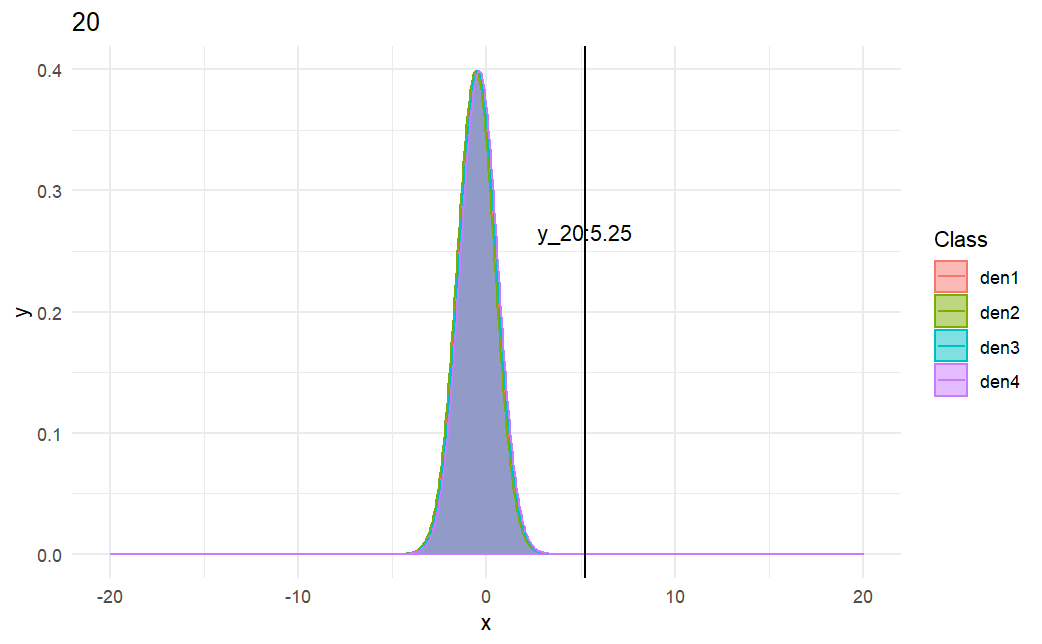
\includegraphics[width=2.7in]{img/test1-rhosame1.png}\\
			\vspace{0.02cm}
			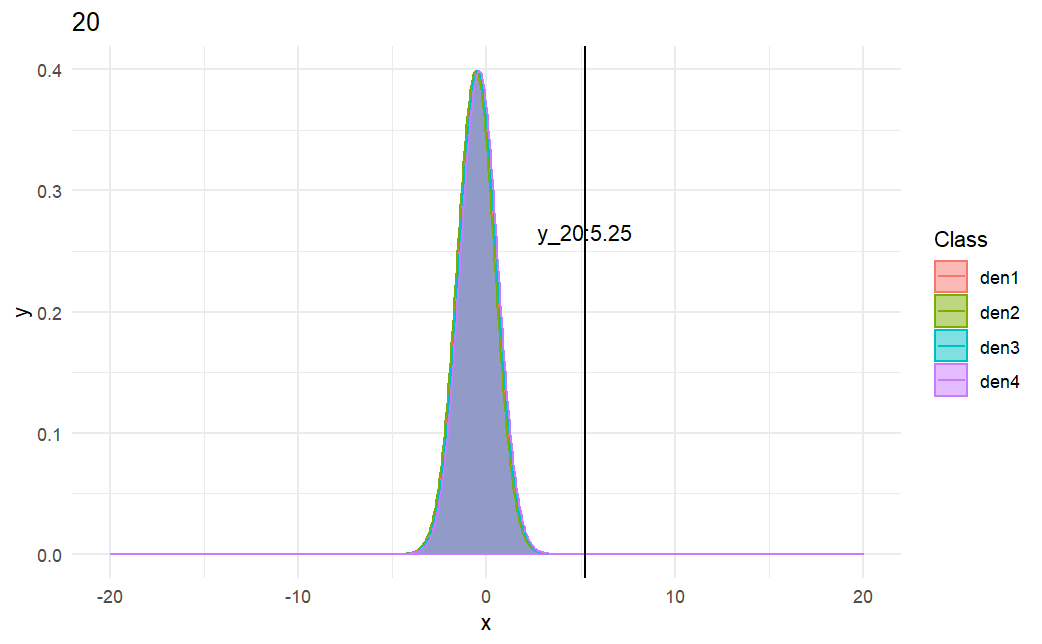
\includegraphics[width=2.7in]{img/test1-rhodiff1.png}\\
			\vspace{0.02cm}
		\end{minipage}%
	}%
	\subfigure{
	\begin{minipage}[t]{0.33\linewidth}
		\centering
		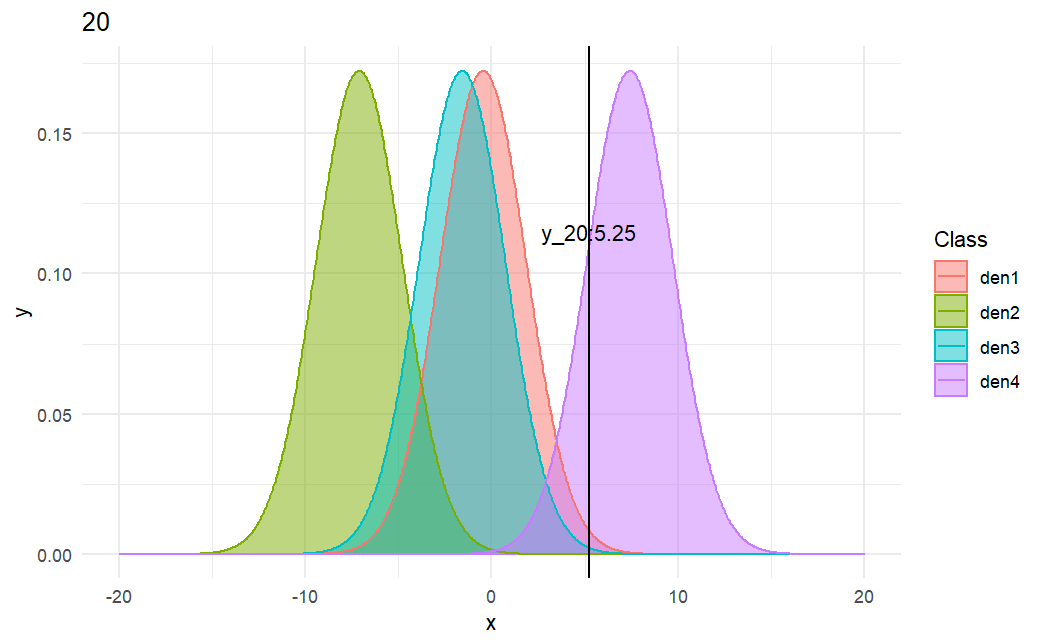
\includegraphics[width=2.7in]{img/test1-rhosame2.png}\\
		\vspace{0.02cm}
		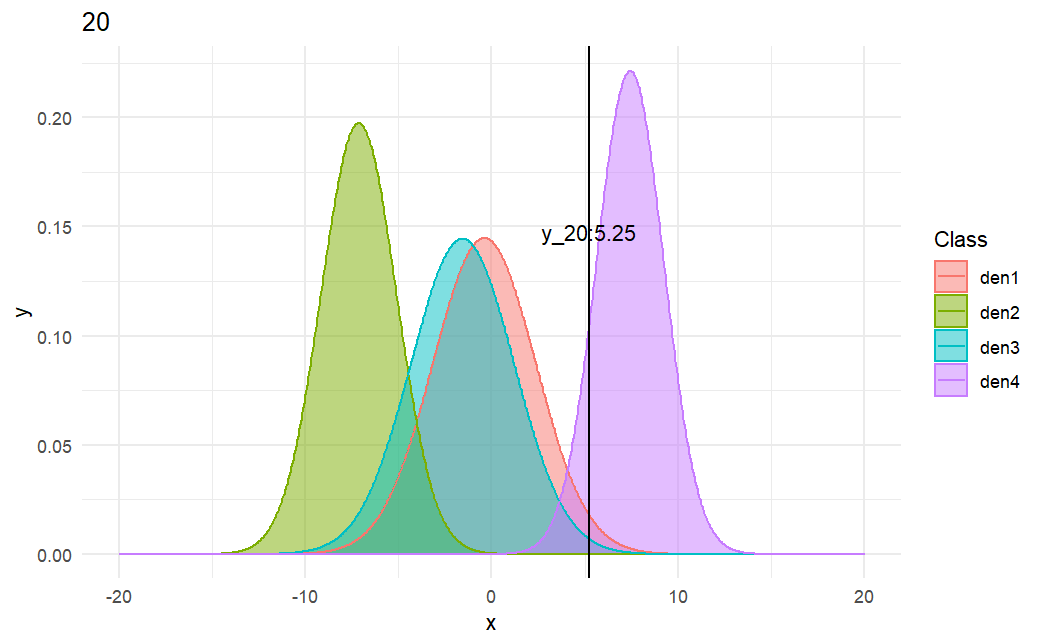
\includegraphics[width=2.7in]{img/test1-rhodiff2.png}\\
		\vspace{0.02cm}
	\end{minipage}%
	}%
	\subfigure{
	\begin{minipage}[t]{0.33\linewidth}
		\centering
		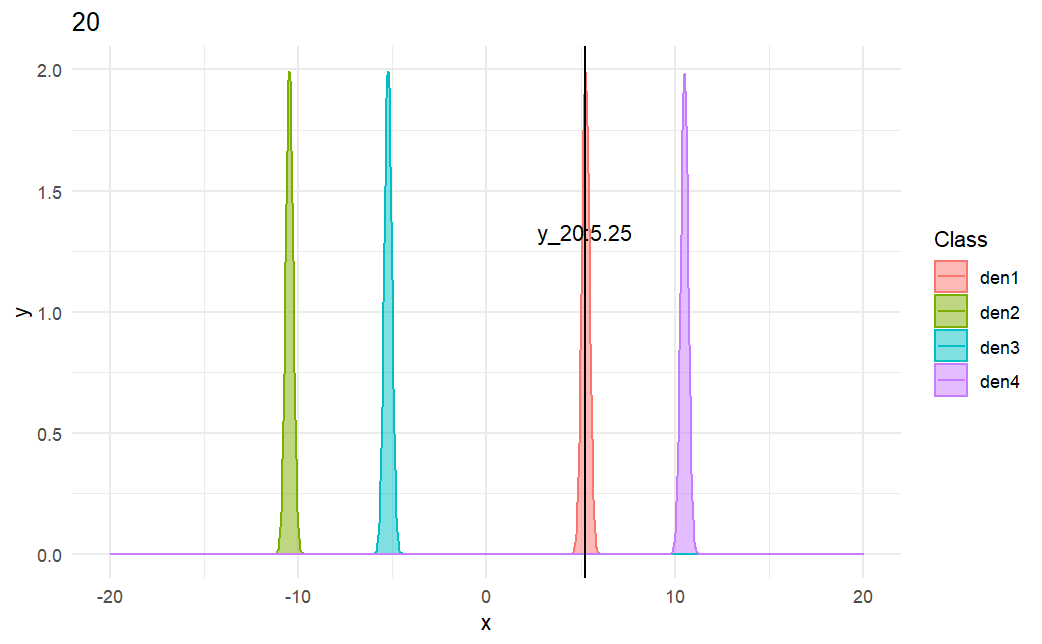
\includegraphics[width=2.7in]{img/test1-rhosame3.png}\\
		\vspace{0.02cm}
		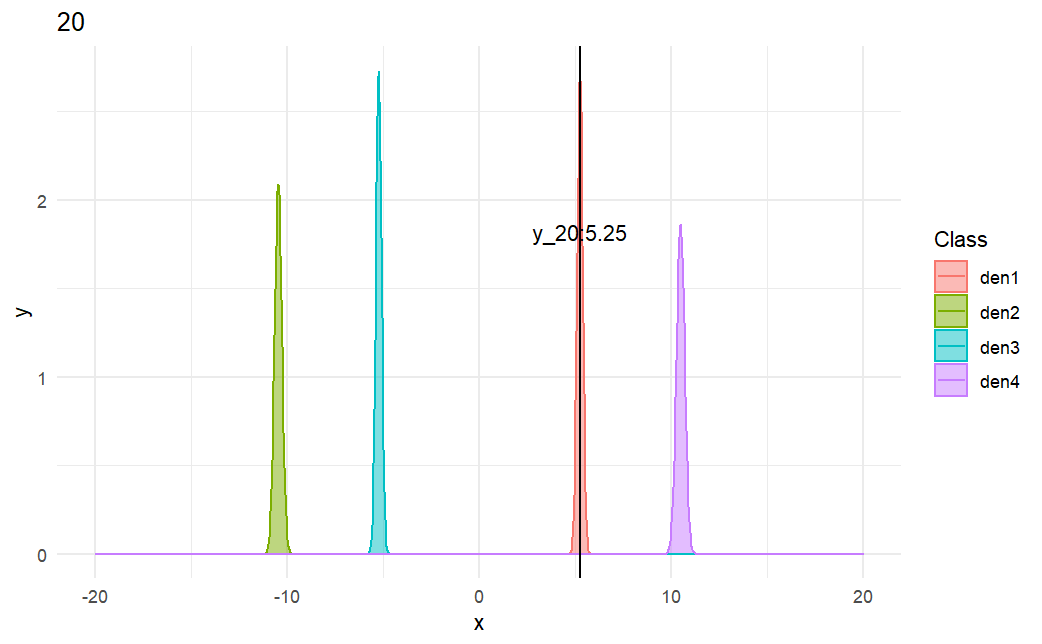
\includegraphics[width=2.7in]{img/test1-rhodiff3.png}\\
		\vspace{0.02cm}
	\end{minipage}%
	}%
	\centering
	\caption{简单设定下各类别分布随迭代轮数变化图(样本 20 为例,第一行为相同类别共用 $\rho$ 的设定,第二行为各类别分别更新各自 $\rho_k$ 的设定)}
	\vspace{-0.2cm}
	\label{fig:simple-vis}
\end{figure*}




\section{Simple Set2-Two Part}

\subsection{Estimation}

该部分本质上依旧是不包含交互项的多分类回归问题,在类别内部有

\begin{equation}
	Y_i = X_i^T\beta_k + Z_i^T\alpha_k, if\ i\in Class\ k
\end{equation}

其中 $\beta_k \in \mathbb{R}^p$,$\alpha_k \in \mathbb{R}^q$,若记 $\tilde X_i^T = (X_i^T, Z_i^T), \theta_k^T = (\beta_k^T, \alpha_k^T)$ 可以将模型改写为 $Y_i = \tilde X_i^T\theta_k$,此时完全退化为最简单线性设定,本部分的重点在于验证两部分依次各自更新迭代公式的正确性。

对于类别 $k$,可以对不同参数写出优化目标,计算时依次迭代即可。

\paragraph{Estimate $\beta_k$}

\begin{equation}
	\begin{aligned}
		\text{min}\qquad l_k &=  \displaystyle\sum_{i=1}^{n}q_{C_i}(k)\left(y_i - X_i^T \beta_k - Z_i^T \alpha_k\right) \\
		&= (y^{\beta_k} - X\beta_k)^T W_k (y^{\beta_k} - X\beta_k)
	\end{aligned}
\end{equation}

其中 $W_k = diag(q_{C_1}(k),...,q_{C_n}(k))$,则 $\beta_k$ 的估计值为

\begin{equation}
	\hat \beta_k = (X^{T} W_k X)^{-1} X^{T} W_k y^{\beta_k}
\end{equation}


\paragraph{Estimate $\alpha_k$}

\begin{equation}
	\begin{aligned}
		\text{min}\qquad l_k &=  \displaystyle\sum_{i=1}^{n}q_{C_i}(k)\left(y_i - X_i^T \beta_k - Z_i^T \alpha_k\right) \\
		&= (y^{\alpha_k} - Z\alpha_k)^T W_k (y^{\alpha_k} - Z\alpha_k)
	\end{aligned}
\end{equation}

$\alpha_k$ 的估计值为

\begin{equation}
	\hat \alpha_k = (Z^T W_k Z)^{-1}Z^T W_k y^{\alpha_k}
\end{equation}

值得注意的是,将两部分参数当做一体的方法更新公式 \ref{eq:two-part1} 与分别更新 $\beta_k,\alpha_k$ 的公式 \ref{eq:two-part2} 并不等价。公式 \ref{eq:two-part1} 中 $\beta_k$ 的更新不依赖于当前 $\alpha_k$ 的取值,反之亦反;而公式 \ref{eq:two-part2} 中 $y^{\beta_k} = y - Z\alpha_k,y^{\alpha_k} = y - X\beta_k$,$\beta_k$ 与 $\alpha_k$ 的更新相互依赖。直观理解上来看,二者计算目标不同,推导方法参照分块矩阵求逆。
\begin{equation}
	\left(\begin{array}{c}
		\hat{\beta}_{k} \\
		\hat{\alpha}_k
	\end{array}\right) = \left((X\ Z)^TW_k (X\ Z)\right)^{-1}(X\ Z)^T W_k y
\label{eq:two-part1}
\end{equation}

\begin{equation}
	\left\{\begin{array}{l}
		\hat{\beta}_{k}=  (X^{T} W_k X)^{-1} X^{T} W_k y^{\beta_k}\\
		\hat{\alpha}_{k}= (Z^T W_k Z)^{-1}Z^T W_k y^{\alpha_k}
	\end{array}\right.
	\label{eq:two-part2}
\end{equation}

\subsection{Numerical Setting}

令 $p=4,q=3$ 四个类别真实参数设置见表 \ref{tb:coef_true_twopart}

\begin{table}[h]
	\centering
	\caption{两部分参数设定}
	\begin{tabular}{ccccc}
		\toprule
		& Comp.1 & Comp.2 & Comp.3 & Comp.4 \\
		\midrule
		$\beta_{k1}$  & -2      & -1      & 1      & 2     \\
		$\beta_{k2}$  & -2      & -1      & 1      & 2     \\
		$\beta_{k3}$  & 0      & 0      & 0      & 0      \\
		$\beta_{k4}$  & 0      & 0      & 0      & 0      \\
		$\alpha_{k1}$  & -2      & -1      & 1      & 2      \\
		$\alpha_{k2}$  & -2      & -1      & 1      & 2      \\
		$\alpha_{k3}$  & 0      & 0      & 0      & 0      \\
		\bottomrule
	\end{tabular}
	\label{tb:coef_true_twopart}
\end{table}

\subsection{Results}

如果根据 $Y_i = \tilde X_i^T\theta_k$ 使用最简情况方法进行求解,可收敛,但初始值的设置需要比较小心。当初始值为一组来自 $N(0,0.1)$ 的随机数时候依旧很快(27轮左右)收敛到真值,但若抽样正态分布方差较大,会出现参数估计不再变化但未收敛到真值的情况。



\section{Simple Set3-Interaction}

\subsection{Estimation}

以上为有分组的简单回归情况,现考虑原模型的协变量构成,即:$X,Z,W$(对应回归参数为 $\beta, \alpha, \eta$,其中 $\eta$ 又由 $\beta,\gamma$ 计算得到,真实需要更新的参数为 $\beta, \alpha, \gamma$),其中 $W$ 为交互项,$Z$ 为环境相关自变量,$X$ 为基因相关自变量。 
考虑加入交互项,目标函数 $\mu_{ik}$ 的成分发生变化,影响和 $\beta,\gamma$ 相关的求解。不影响 $\alpha$ 的求解。

与式 \ref{eq:l} 形式类似有

\begin{equation}
	\begin{aligned}
		l &= \displaystyle\sum_{i=1}^{n}\sum_{k=1}^{K}q_{C_i}(k)\left(C - \frac{\rho^2}{2}(y_i - \mu_{ik})^2 \right) \\
		&= \displaystyle\sum_{i=1}^{n}\sum_{k=1}^{K}q_{C_i}(k)\left(C - \frac{\rho^2}{2}(y_i - X_i^T \beta_k - Z_i^T \alpha_k - W_i^T \eta_k)^2 \right)
	\end{aligned}
\end{equation}

为了方便从交互项中按照不同需要拆分出系数,验证以下几种表达形式的等价(数值验证)

\begin{equation}
	\begin{aligned}
		W_i^T \eta_i &= W_i^T(I_q\otimes\beta_k \odot \gamma_k) \\
		&= \sum_{s=1}^{q}W_i^{(s)T}\beta_k\odot \gamma_{ks} \\
		&= (\sum_{s=1}^{q}W_i^{(s)}\odot \gamma_{ks})^T \beta_k \\
		&= (W_i \odot (I_q \otimes \beta_k))^T \gamma_k
	\end{aligned}
\label{eq:same}
\end{equation}

对于类别 $k$,可以对不同参数写出优化目标

\paragraph{Estimate $\alpha_k$}

\begin{equation}
	\begin{aligned}
		\text{min}\qquad l_k &=  \displaystyle\sum_{i=1}^{n}q_{C_i}(k)\left(y_i - X_i^T \beta_k - Z_i^T \alpha_k - W_i^T \eta_k\right) \\
		&= (y^{\alpha_k} - Z\alpha_k)^T W_k (y^{\alpha_k} - Z\alpha_k)
	\end{aligned}
\end{equation}

其中 $y_i^{\alpha_k} = y_i - X_i^T \beta_k - W_i^T \eta_k$, $y^{\alpha_k} = (y_1^{\alpha_k},...,y_n^{\alpha_k})^T$,$W_k = diag(q_{C_1}(k),...,q_{C_n}(k))$,则 $\alpha_k$ 的估计值为

\begin{equation}
	\hat \alpha_k = (Z^T W_k Z)^{-1}Z^T W_k y^{\alpha_k}
\end{equation}

\paragraph{Estimate $\beta_k$}

\begin{equation}
	\begin{aligned}
		\text{min}\qquad l_k &=  \displaystyle\sum_{i=1}^{n}q_{C_i}(k)\left(y_i - X_i^T \beta_k - Z_i^T \alpha_k - W_i^T \eta_k\right) \\
		&= (y^{\beta_k} - X^{\beta_k}\beta_k)^T W (y^{\beta_k} - X^{\beta_k}\beta_k)
	\end{aligned}
\end{equation}

其中 $X^{\beta_k} = (X^{\beta_k}_1,...,X^{\beta_k}_n)^T \in \mathbb{R}^{n\times p}$, $X^{\beta_k}_i = X_i + (\sum_{s=1}^{q}W_i^{(s)}\odot\gamma_{ks}) \in \mathbb{R}^{p\times 1}$, $y_i^{\beta_k} = y_i - Z_i^T\alpha_k, y_i^{\beta_k} = (y_1^{\beta_k},...,y_n^{\beta_k})^T$,$W_k = diag(q_{C_1}(k),...,q_{C_n}(k))$,则 $\beta_k$ 的估计值为

\begin{equation}
	\hat \beta_k = (X^{\beta_k T} W_k X^{\beta_k})^{-1} X^{\beta_k T} W_k y^{\beta_k}
\end{equation}

\paragraph{Estimate $\gamma_k$}

\begin{equation}
	\begin{aligned}
		\text{min}\qquad l_k &=  \displaystyle\sum_{i=1}^{n}q_{C_i}(k)\left(y_i - X_i^T \beta_k - Z_i^T \alpha_k - W_i^T \eta_k\right) \\
		&= (y^{\gamma_k} - X^{\gamma_k}\gamma_k)^T W (y^{\gamma_k} -  X^{\gamma_k}\gamma_k)
	\end{aligned}
\end{equation}

其中 $X^{\gamma_k} = (X^{\gamma_k}_1,...,X^{\gamma_k}_n)^T \in \mathbb{R}^{n\times pq}$, $X^{\gamma_k}_i = W_i\odot (I_q \otimes \beta_k) \in \mathbb{R}^{pq\times 1}$, $y_i^{\gamma_k} = y_i - X_i^T\beta_k - Z_i^T\alpha_k, y_i^{\gamma_k} = (y_1^{\gamma_k},...,y_n^{\gamma_k})^T$,$W_k = diag(q_{C_1}(k),...,q_{C_n}(k))$,则 $\gamma_k$ 的估计值为

\begin{equation}
	\hat \gamma_k = (X^{\gamma_k T} W_k X^{\gamma_k})^{-1} X^{\gamma_k T} W_k y^{\gamma_k}
\end{equation} 

$X^{\beta_k}$ 依赖于当前 $\gamma_k$ 估计值,$X^{\gamma_k}$ 也依赖于当前 $\beta_k$ 的估计值。有交互项的情况不再可以直接化为最简单的线性回归情况,即不可以一次性算出一轮参数的更新。综上,更新总结如式 \ref{eq:interaction}


\begin{equation}
	\left\{\begin{array}{l}
		\hat{\beta}_{k} = (X^{\beta_k T} W_k X)^{-1} X^{\beta_k T} W_k y^{\beta_k}\\
		\hat{\alpha}_{k} = (Z^T W_k Z)^{-1}Z^T W_k y^{\alpha_k}\\
		\hat{\gamma}_{k} = (X^{\gamma_k T} W_k X)^{-1} X^{\gamma_k T} W_k y^{\gamma_k}
	\end{array}\right.
	\label{eq:interaction}
\end{equation}

\subsection{Numerical Setting}

1. 主要实验设置:$p=4,q=3,n=200,K=4$,真实参数设置如表 \ref{tb:coef_true} 

2. 辅助实验设置:$p=2,q=2,n=200,K=4$,真实参数设置如表 \ref{tb:coef_true_nonzero}.

\subsection{Package Results}

注意在有交互项的模型中,包得到的结果和上述更新不同。形式 

\begin{equation}
	\begin{aligned}
		y_i &= \displaystyle\sum_{k=1}^{K} q_{C_i}(k) \left(X_i^T \beta_k + Z_i^T \alpha_k + W_i^T \eta_k\right) \\
		&= \displaystyle\sum_{k=1}^{K} q_{C_i}(k) \left(X_i^T \beta_k + Z_i^T \alpha_k + (W_i \odot (I_q \otimes \beta_k))^T \gamma_k\right)
	\end{aligned}
\end{equation}

加权最小二乘法得到的是 $\beta_k, \alpha_k, \gamma_k$ 的更新,$\eta_k$ 是根据其他参数计算出来的。而直接用包得到的参数为 $\beta_k, \alpha_k, \eta_k$, $\gamma_k$ 需要再计算。当然也可以重新定义 $\gamma_k$ 相关的自变量为 $W_i \odot (I_q \otimes \beta_k)$,但该表达式包含 $\beta_k$。

\textit{fmrs}:$p=2,q=2$ 效果不好

\textit{flexmix}:$p=2,q=2$ 计算正确

\begin{table}[h]
	\centering
	\begin{tabular}{ccccc}
		\toprule
		& Comp.1 & Comp.2 & Comp.3 & Comp.4 \\
		\midrule
		$\beta_{k1}$   & 2      & 2      & -2     & -2     \\
		$\beta_{k2}$   & 2      & 2      & -2     & -2     \\
		\midrule
		$\alpha_{k1}$  & 2      & 2      & -2     & -2     \\
		$\alpha_{k2}$  & 2      & 2      & -2     & -2     \\
		\midrule
		$\gamma_{k1}$  & 3      & 1      & -1     & -3     \\
		$\gamma_{k2}$  & 3      & 1      & -1     & -3     \\
		$\gamma_{k3}$  & 3      & 1      & -1     & -3     \\
		$\gamma_{k4}$  & 3      & 1      & -1     & -3     \\
		\bottomrule
	\end{tabular}
	\label{tb:coef_true_nonzero}
\end{table}

\begin{table}[h]
	\centering
	\begin{tabular}{ccccc}
		\toprule
		& Comp.1 & Comp.2 & Comp.3 & Comp.4 \\
		\midrule
		$\beta_{k1}$   & 2      & 2      & -2     & -2     \\
		$\beta_{k2}$   & 2      & 2      & -2     & -2     \\
		$\beta_{k3}$   & 0      & 0      & 0      & 0      \\
		$\beta_{k4}$   & 0      & 0      & 0      & 0      \\
		\midrule
		$\alpha_{k1}$  & 2      & 2      & -2     & -2     \\
		$\alpha_{k2}$  & 2      & 2      & -2     & -2     \\
		$\alpha_{k3}$  & 0      & 0      & 0      & 0      \\
		\midrule
		$\gamma_{k1}$  & 3      & 1      & -1     & -3     \\
		$\gamma_{k2}$  & 3      & 1      & -1     & -3     \\
		$\gamma_{k3}$  & 3      & 1      & -1     & -3     \\
		$\gamma_{k4}$  & 3      & 1      & -1     & -3     \\
		$\gamma_{k5}$  & 0      & 0      & 0      & 0      \\
		$\gamma_{k6}$  & 0      & 0      & 0      & 0      \\
		$\gamma_{k7}$  & 0      & 0      & 0      & 0      \\
		$\gamma_{k8}$  & 0      & 0      & 0      & 0      \\
		$\gamma_{k9}$  & 0      & 0      & 0      & 0      \\
		$\gamma_{k10}$ & 0      & 0      & 0      & 0      \\
		$\gamma_{k11}$ & 0      & 0      & 0      & 0      \\
		$\gamma_{k12}$ & 0      & 0      & 0      & 0     \\
		\bottomrule
	\end{tabular}
	\label{tb:coef_true}
\end{table}

直接计算流程类似于算法 \ref{alg:simplest},固定其他参数依次更新 $\beta_k, \alpha_k, \gamma_k$ 即可。

\subsection{Iteration Results}

总结实验经验结果如下:
\begin{enumerate}
	\item 迭代过程中需要实时使用最新结果,而不是在一轮迭代中统一使用上一轮结果,这样可以避免参数距离真值的距离来回震荡,形成两三条曲线;
	\item 矩阵求逆出现特征值过小情况应加上一个小数乘以对角阵,小数取 0.1 已经足够大,否则会影响参数估计;
	\item 更新单个参数或更新一对参数检验时,定位问题所在是 $\beta_k$ 和 $\gamma_k$ 的交互项;
	\item 原始问题非凸,依赖初始值,固定初始化方法相比随机初始化较稳定。
\end{enumerate}

\subsubsection{One Class}

模型不收敛有两个的可能:(1)参数迭代估计过程中出错;(2)后验概率相关。为逐一排除错误,首先去除后验概率的影响,先对单类别进行实验。取不收敛异常样例(seed 11,K4)进行分析,选取固定初始化方法和 7 组随机初始化,得到收敛曲线及使用对应参数进行回归估计得到残差分布图与 MSE 如图 \ref{fig:seed11k4_seeds}.

\begin{figure}
	\centering
	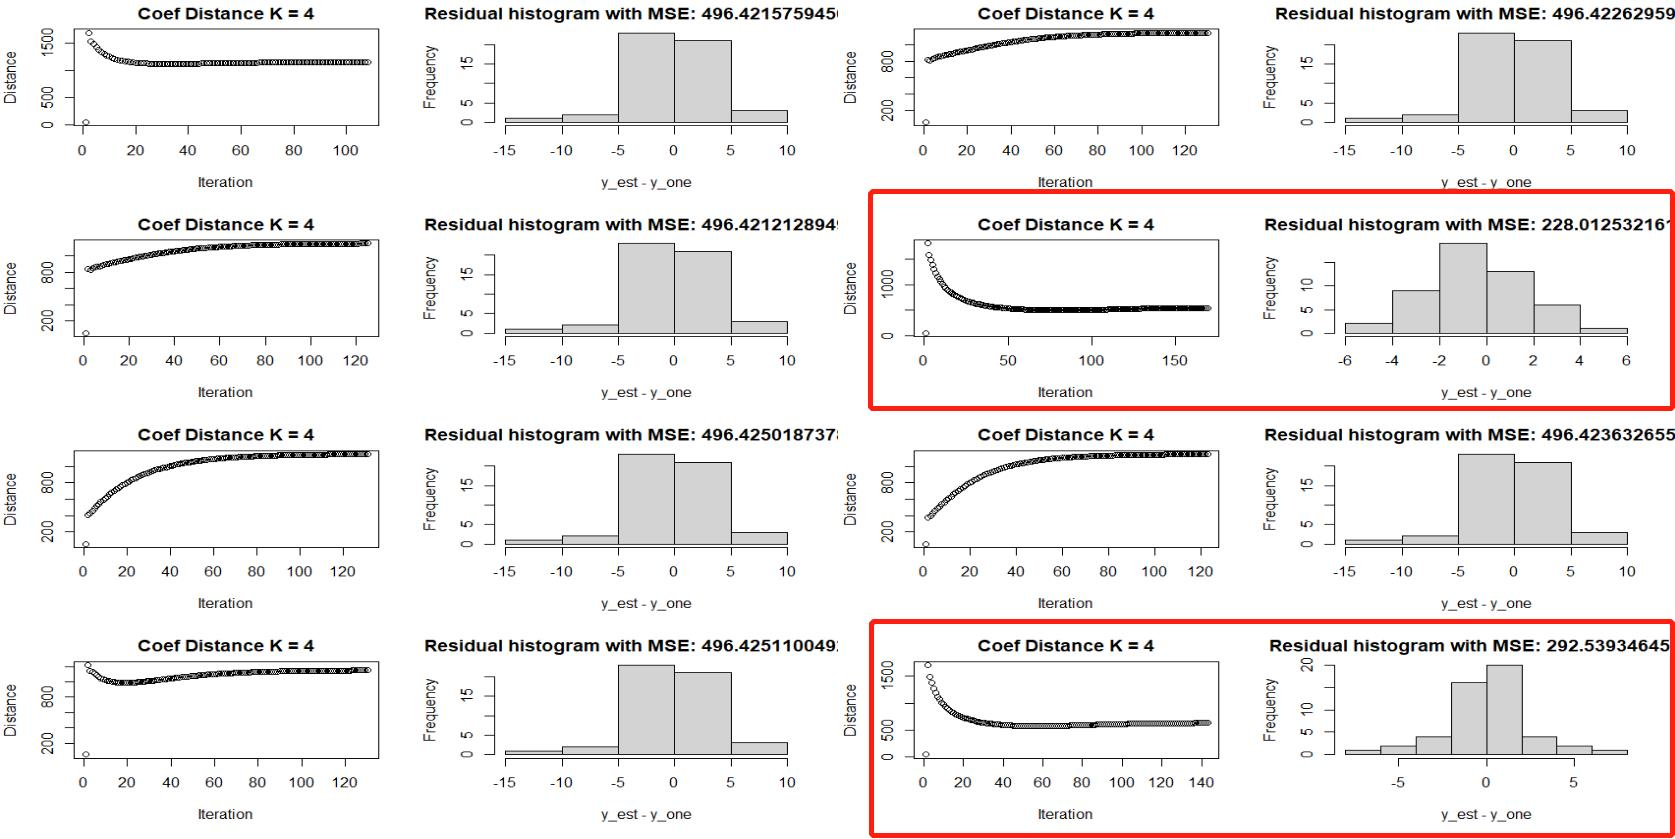
\includegraphics[width=\textwidth]{img/seed11k4_seeds.jpg}
	\caption{多组初始化下,参数到真值距离随迭代轮数的变化(seed 11,K4)}
	\label{fig:seed11k4_seeds}
\end{figure}

随机设置 200 组(199 组$N(0,0.01)$初始值+1组固定初始值),得到的参数距离真值的距离总结如图 \ref{fig:seed11_200}.

\begin{figure*}
	\centering
	\subfigure{
		\begin{minipage}[t]{0.45\linewidth}
			\centering
			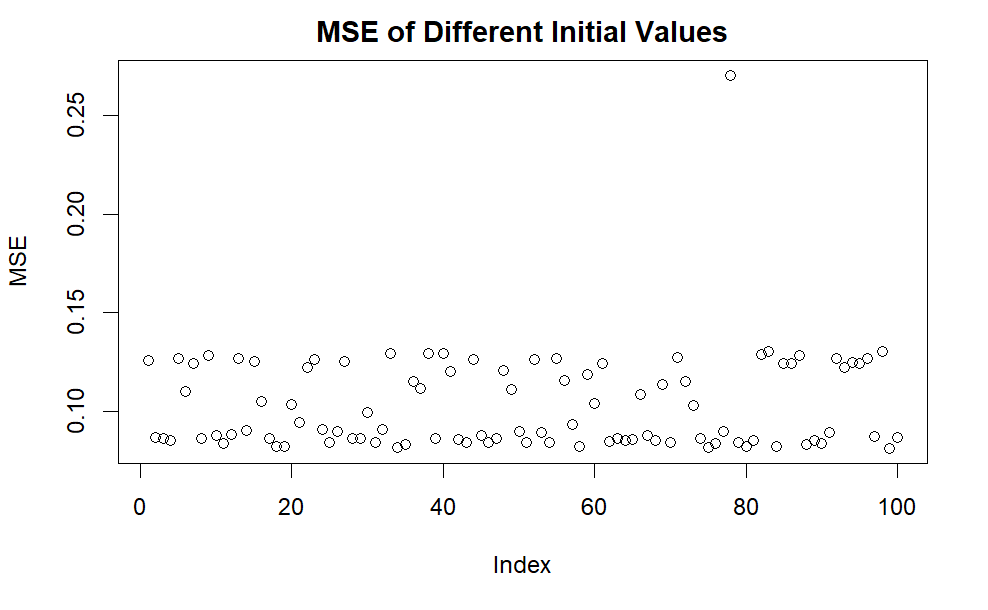
\includegraphics[width=3in]{img/seed11k1_200.png}\\
			\vspace{0.02cm}
			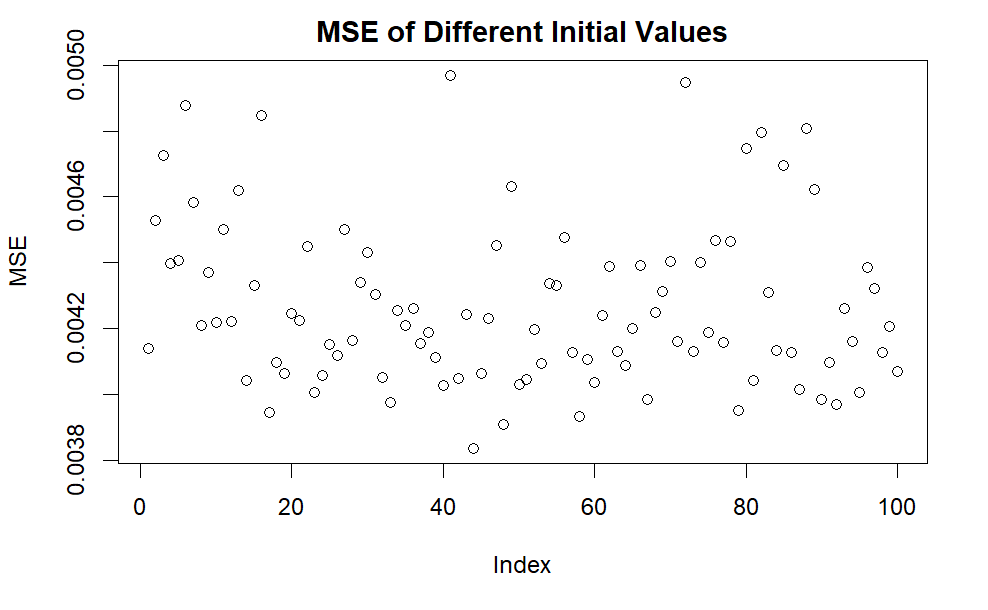
\includegraphics[width=3in]{img/seed11k3_200.png}\\
			\vspace{0.02cm}
		\end{minipage}%
	}
	\subfigure{
		\begin{minipage}[t]{0.45\linewidth}
			\centering
			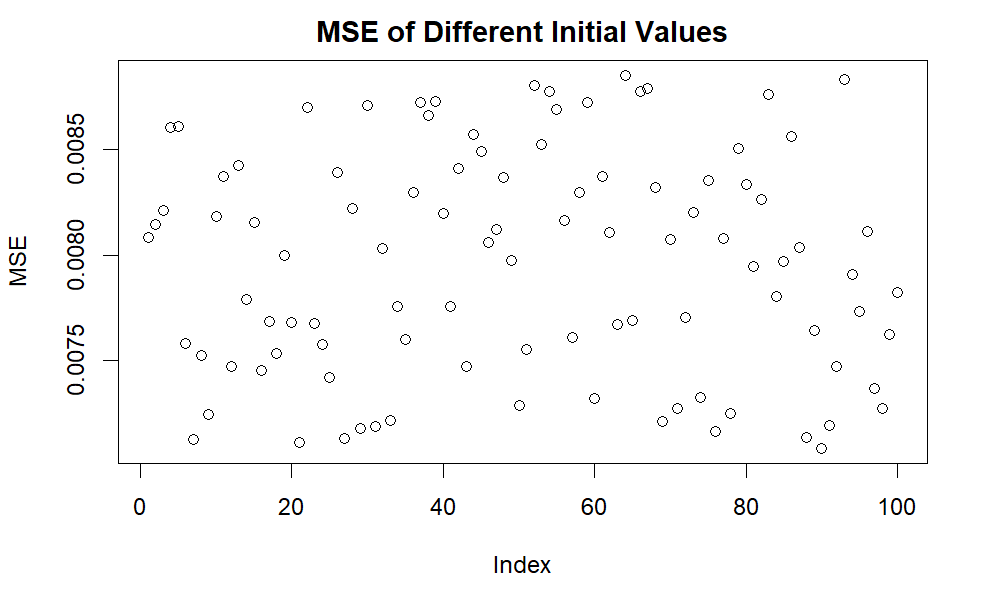
\includegraphics[width=3in]{img/seed11k2_200.png}\\
			\vspace{0.02cm}
			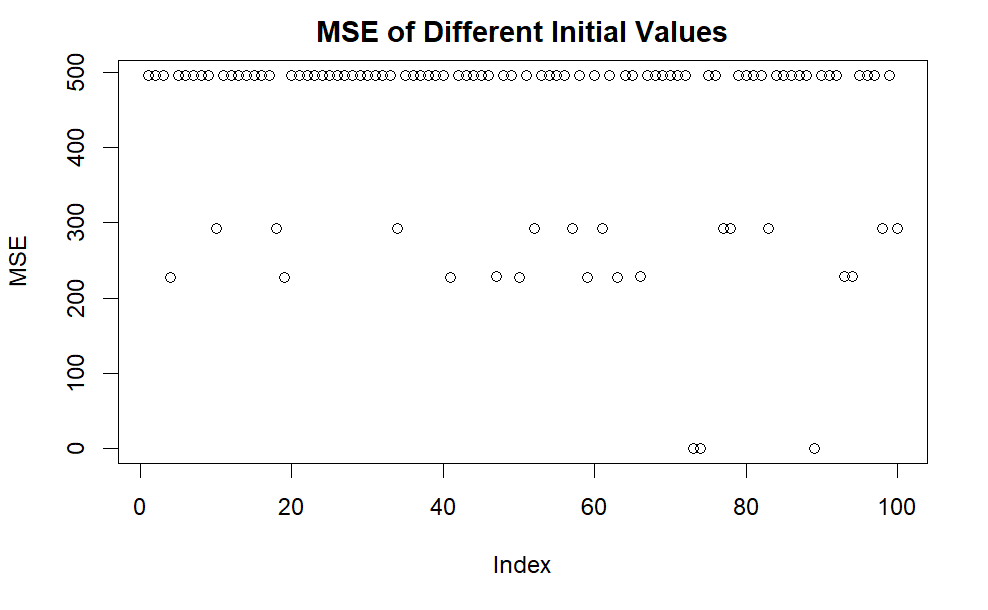
\includegraphics[width=3in]{img/seed11k4_200.png}\\
			\vspace{0.02cm}
		\end{minipage}%
	}
	\caption{200 组初始化下最终得到的 MSE(seed 11,K 1,2,3,4,注意纵坐标尺度差异)}
	\vspace{-0.2cm}
	\label{fig:seed11_200}
\end{figure*}

当前做法为,在迭代开始前得到 200 组初始值,依次代入循环,若某一次使用其结果进行回归得到的 MSE 小于临界值(暂时设置为 1),则停止尝试其他初值,认为已经得到比较好的结果;如果试遍所有 200 个初始值依旧没有得到足够小的 MSE,则选取相对较好的结果,此时结果依旧不理想,应回查,现有实验中尚未遇到这种情况,最多 72 次初始值尝试后就得到理想 MSE。

\subsubsection{Multiple Class-Fixed $q_{C_i}$}

多组初始值的设置行之有效,将单类实验嵌入多类别框架,即恢复样本属于不同类别的设定,但已知其真值分组,此时多分类实验等价于同时进行多组单类实验,各个类别的参数互不影响,但只有当每个类别都正常收敛时才会认为一次多类实验成功。结果展示如图 \ref{fig:seed111},\ref{fig:seed14},\ref{fig:seed11}。

\begin{figure}
	\centering
	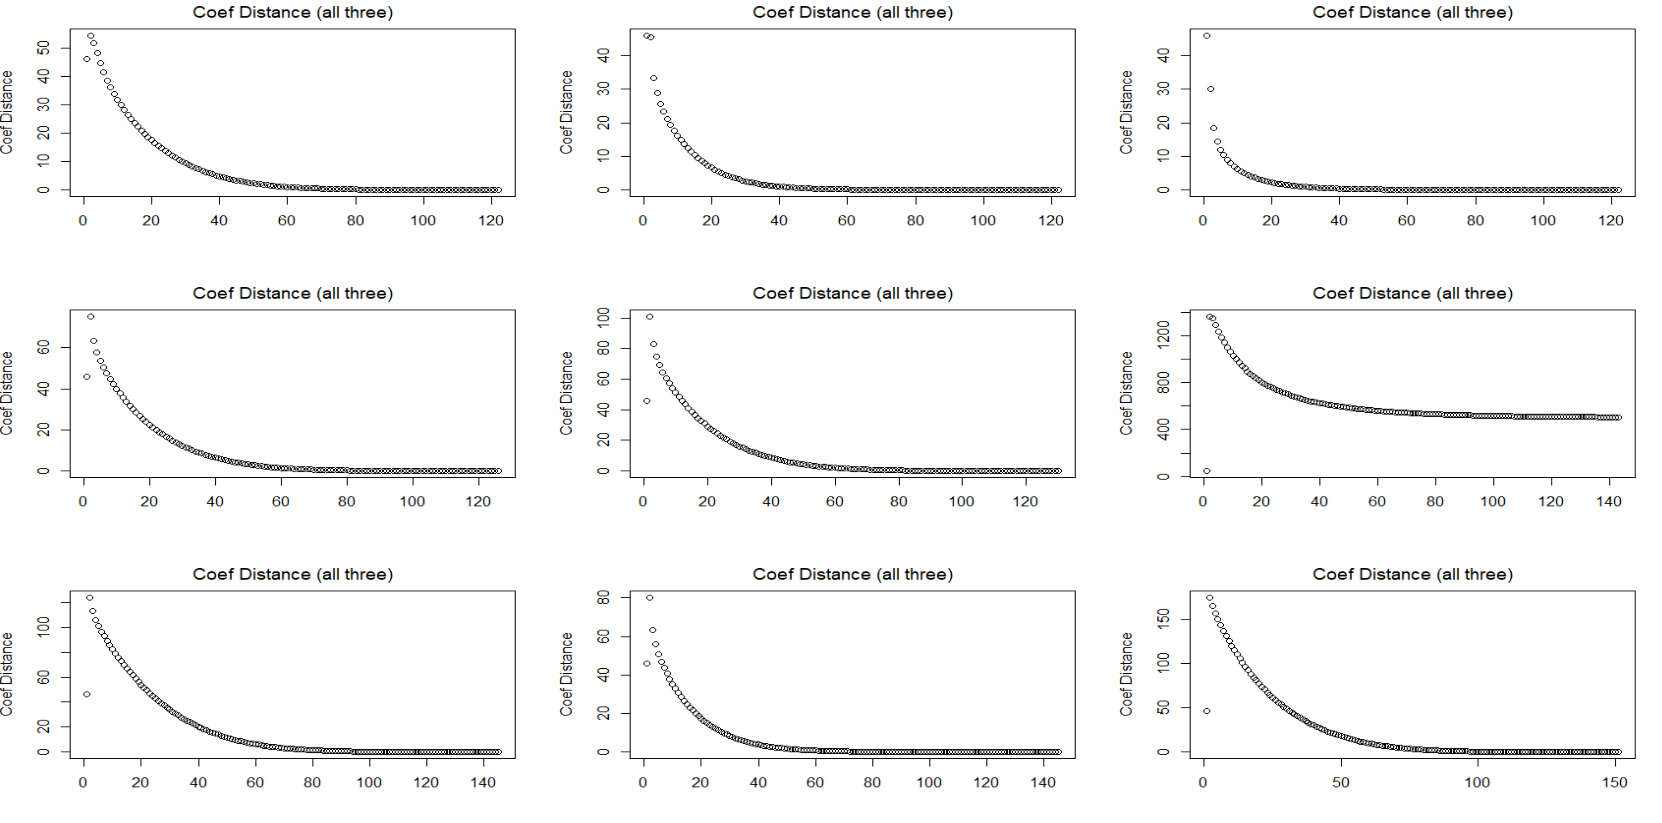
\includegraphics[width=\textwidth]{img/seed111.png}
	\caption{多组初始化下,参数到真值距离随迭代轮数的变化(seed 111)}
	\label{fig:seed111}
\end{figure}

\begin{figure}
	\centering
	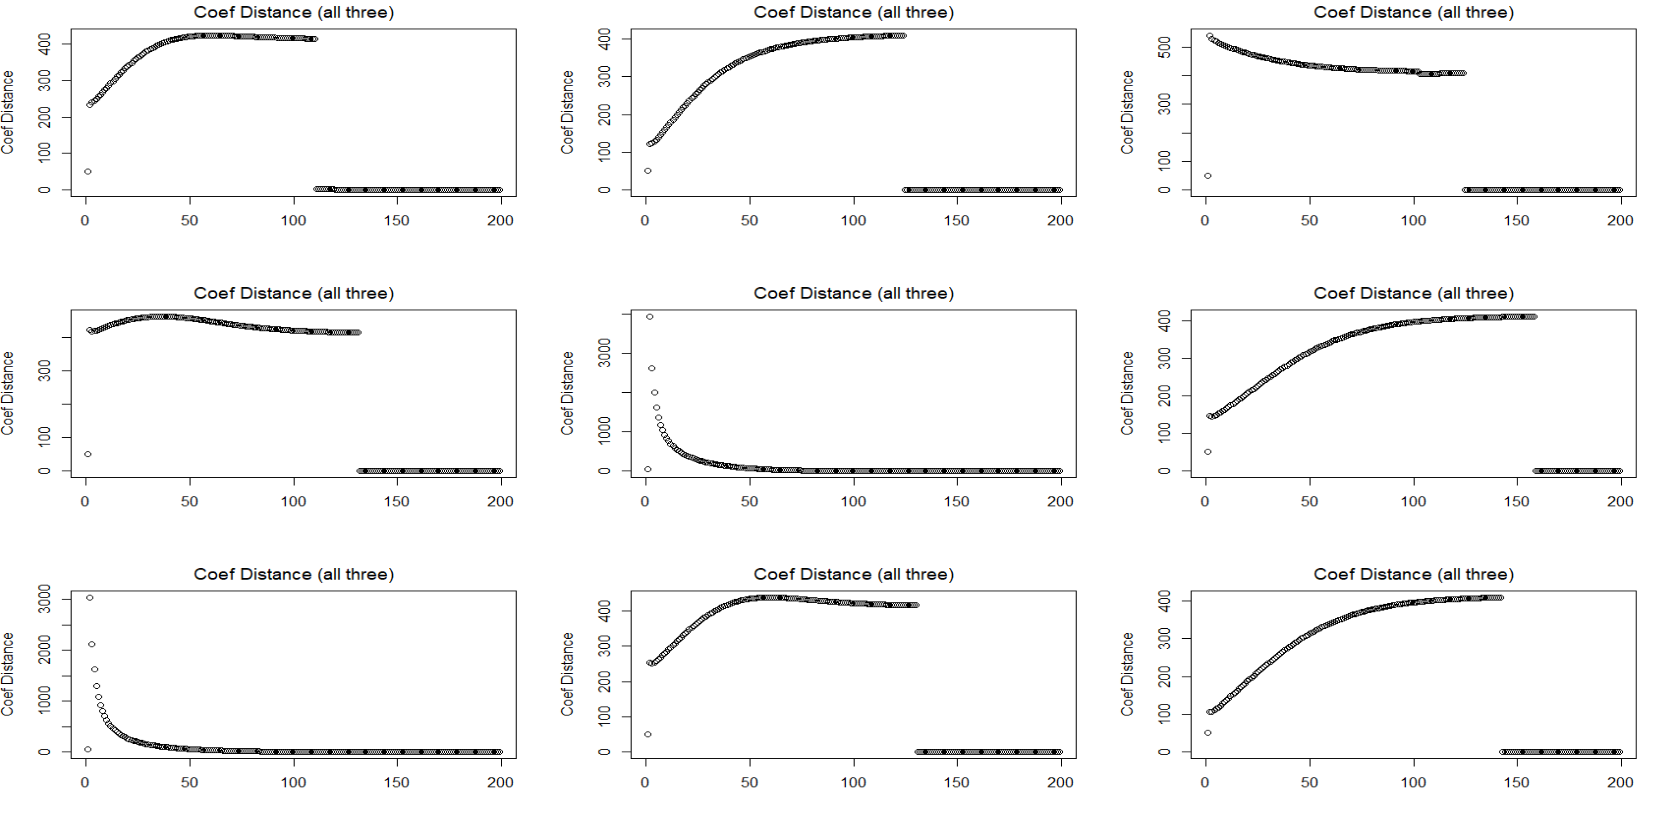
\includegraphics[width=\textwidth]{img/seed14.png}
	\caption{多组初始化下,参数到真值距离随迭代轮数的变化(seed 14)}
	\label{fig:seed14}
\end{figure}

\begin{figure}
	\centering
	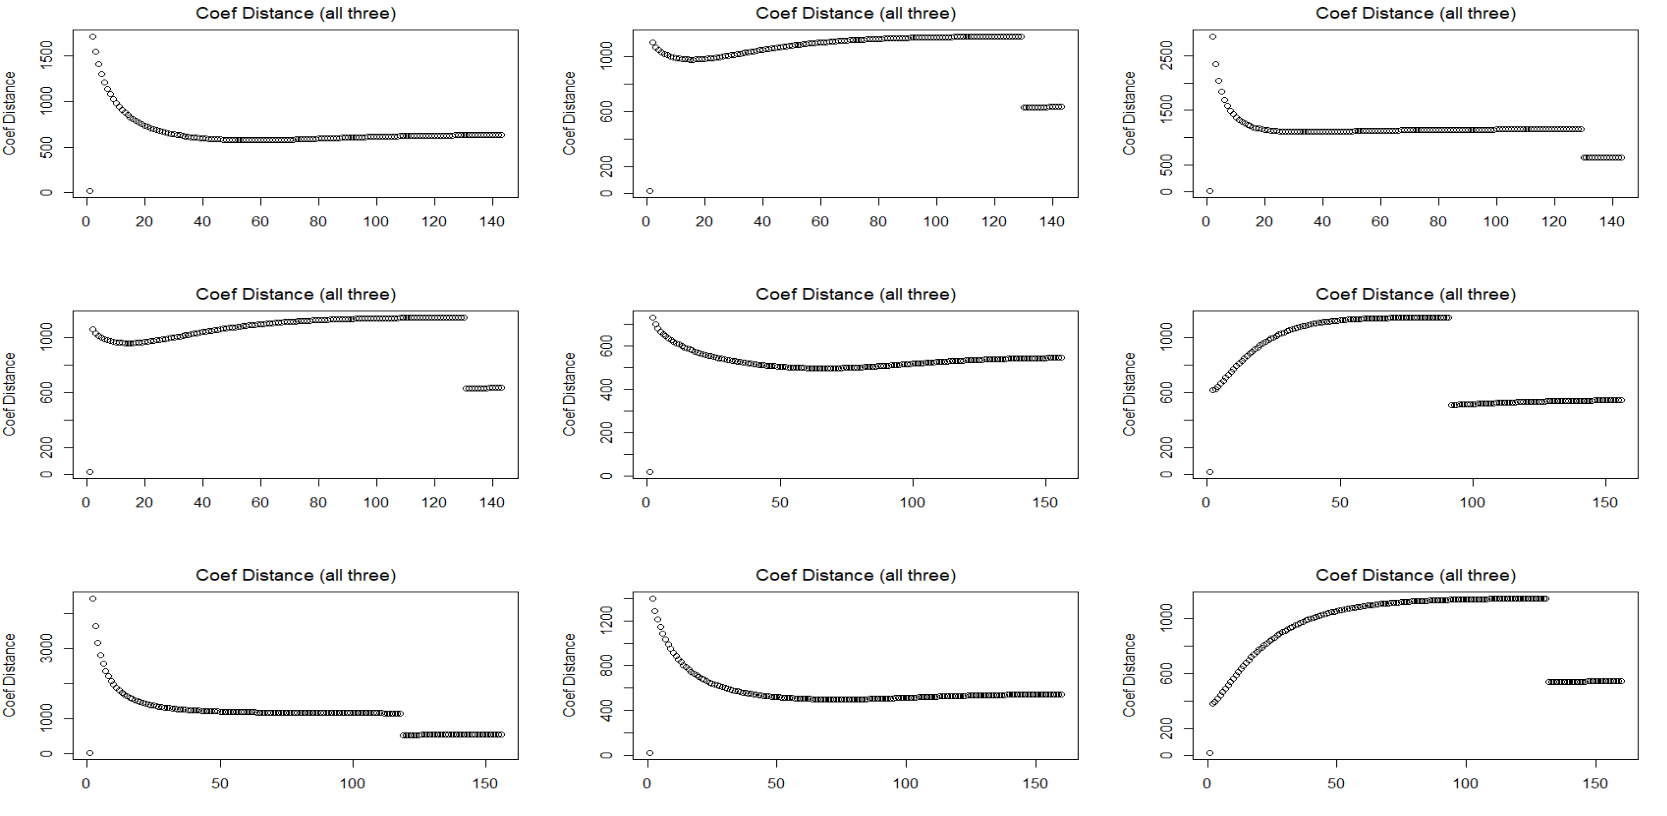
\includegraphics[width=\textwidth]{img/seed11.png}
	\caption{多组初始化下,参数到真值距离随迭代轮数的变化(seed 11)}
	\label{fig:seed11}
\end{figure}

此处实验样例均为之前单分类至少有一个分类异常的数据,seed 11 生成的数据较难估计参数,9 组初始值不足以估计出真实结果,尝试 100 组初始值,使用对应参数估计得到的回归模型 MSE 如图 \ref{fig:seed11}.

\begin{figure}
	\centering
	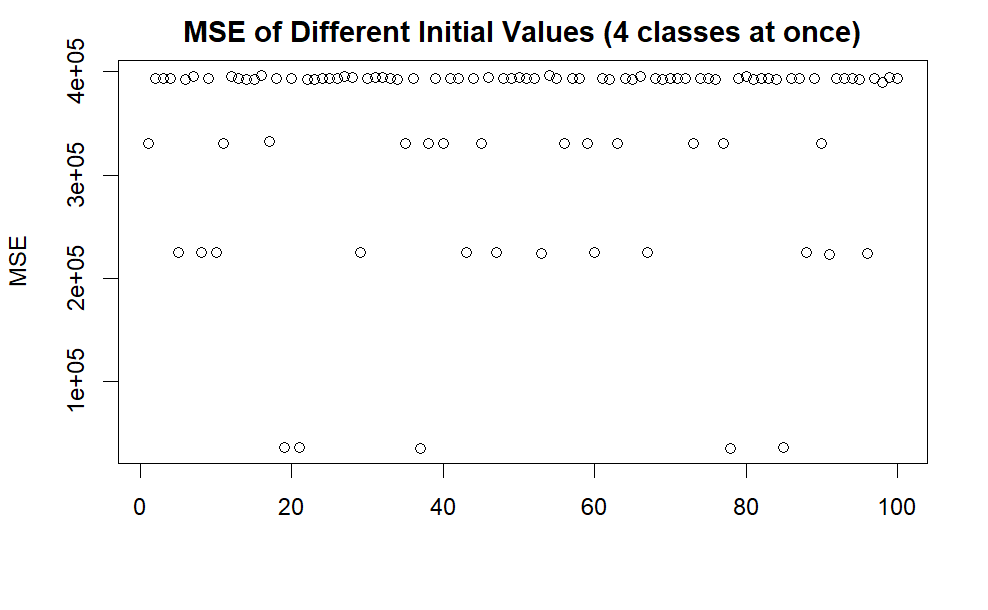
\includegraphics[width=0.8\textwidth]{img/seed11k1234_200.png}
	\caption{100 组初始化下最终得到的 MSE(seed 11,所有分类)}
	\label{fig:seed11}
\end{figure}

值得注意的是,将生成的所有初始值都尝试一遍后再选择最优结果效率低但比较稳妥;MSE 小于临界值的方法不容易找到合适的临界值,比如在图 \ref{fig:seed11} 的例子中,最小的 MSE 是 35883.49,对应的参数估计结果为表 \ref{tb:best_coef_seed11}(真值见表 \ref{tb:coef_true_nonzero}) MSE 数值虽大但收敛到几乎为真值的地方,临界值和数据的尺度有关。

\begin{table}[ht]
	\centering
	\caption{seed 11 数据在 100 组初始值中的最佳收敛结果}
	\vspace{0.2cm}
	\label{tb:best_coef_seed11}
	\begin{tabular}{rrrrr}
		\toprule
		& Class 1 & Class 2 & Class 3 & Class 4 \\ 
		\midrule
		$\beta_{k1}$ & 2.051 & 1.997 & -1.999 & -2.010 \\ 
		$\beta_{k2}$ & 1.980 & 1.998 & -1.996 & -2.015 \\ 
		$\alpha_{k1}$ & 1.985 & 1.996 & -1.996 & -1.998 \\ 
		$\alpha_{k2}$ & 1.994 & 1.994 & -1.994 & -1.999 \\ 
		$\gamma_{k1}$ & 2.911 & 1.002 & -1.000 & -2.983 \\ 
		$\gamma_{k2}$ & 3.033 & 1.000 & -0.999 & -2.976 \\ 
		$\gamma_{k3}$ & 2.931 & 1.002 & -1.000 & -2.985 \\ 
		$\gamma_{k4}$ & 3.026 & 0.999 & -1.000 & -2.978 \\ 
		\bottomrule
	\end{tabular}
\end{table}

\subsubsection{Multiple Class-Unknown $q_{C_i}$}

进一步,取消已知 $q_{C_i}$ 的限制,将各个样本的后验概率估计也加入迭代过程





\clearpage

\section{Test Summary}

\begin{enumerate}
	\item 初始化参数而非后验概率,EM 算法顺序不可倒置否则无法与原包结果进行对比
	\item $\rho$ 的更新方式,按照类别分和不同类别取平均作每个类别 $1/\sigma$ 效果没有明显差别,为了防止某类异常影响整体效果当前各类别有自己的方差。考虑到及时在最终应用场景中,目标类别也不会太多,这样的设定应该不会增加很大计算复杂度,若有需要再进行调整
\end{enumerate}



\newpage
\bibliographystyle{plain}
\bibliography{ref}

\end{document}